% last updated in April 2002 by Antje Endemann
% Based on CVPR 07 and LNCS, with modifications by DAF, AZ and elle, 2008 and AA, 2010, and CC, 2011; TT, 2014

\documentclass[runningheads]{llncs}
\usepackage{graphicx}
\usepackage{amsmath,amssymb} % define this before the line numbering.
\usepackage{ruler}
\usepackage{color}
\usepackage{array}
\usepackage{float}
\usepackage{subfig,caption}
\usepackage{lipsum}
\usepackage{dcolumn}



%\usepackage{subcaption}
\usepackage{comment}
\renewcommand{\arraystretch}{1.1}
\usepackage[width=122mm,left=12mm,paperwidth=146mm,height=193mm,top=12mm,paperheight=217mm]{geometry}
\begin{document}
% \renewcommand\thelinenumber{\color[rgb]{0.2,0.5,0.8}\normalfont\sffamily\scriptsize\arabic{linenumber}\color[rgb]{0,0,0}}
% \renewcommand\makeLineNumber {\hss\thelinenumber\ \hspace{6mm} \rlap{\hskip\textwidth\ \hspace{6.5mm}\thelinenumber}}
% \linenumbers
\pagestyle{headings}
\mainmatter
\def\ECCV14SubNumber{1355}  % Insert your submission number here

\title{Analyzing The Performance of Multilayer Neural Networks for Object Recognition: Supplementary Material} % Replace with your title

\titlerunning{ECCV-14 submission ID \ECCV14SubNumber}

\authorrunning{ECCV-14 submission ID \ECCV14SubNumber}

\author{Anonymous ECCV submission}
\institute{Paper ID \ECCV14SubNumber}


\maketitle


\section{On Using Entropy For Measuring Change in Selectivity}
\subsection{Motivation}
In answer to question -``What happens when a discriminatively pretrained network is fine-tuned" (sec 3 of the main paper) we have used entropy of filters and entropy of layers as a measure of how selective each layer is. The choice of entropy is motivated by: Entropy naturally measures how selective a particular feature is across different classes and not just individual classes. Consequently, entropy has been extensively used in a lot of computer vision applications based on decision trees such as \cite{AmitGeman} \cite{Breiman}. 

\subsection{Method of Entropy Computation}
We presented a natural way of computing entropy of each unit of every layer in sec 2.3 of the paper. We call this Label-Entropy. However, one might also compute entropy of units in other ways. We considered two more such methods as described below.

We define the entropy of a filter with respect to a given set of image-label paris in the following way. Each image, when passed through the convolutional neural network produces a $p \times p$ heatmap of filter responses. (eg p = 6, for a layer 5 filter). Further assume that there are $C$ classes.
\subsubsection{Label Entropy}
\label{sub:def-label-ent}
We vectorize the heatmap into a vector of scores of length $p^2$ and with each element of this vector we associate the class label of the image. Thus, for each image we have a score vector and a label vector of length $p^2$ each. Next, we concatenate score vectors and label vectors from N images into a giant score vector and a giant label vector  of size $Np^2$ each. Now for every score threshold we consider all the labels which have an associated score $\geq$ to this threshold score. The entropy of this set of labels is the entropy of the filter at this threshold. As this threshold changes, entropy traces out a curve which we call as the entropy curve.  

\subsubsection{Weighted Label Entropy}
\label{sub:def-weighted-label-ent}
We vectorize the heatmap into a vector of scores of length $p^2$ and with each element of this vector we associate the class label of the image. Thus, for each image we have a score vector and a label vector of length $p^2$ each. Next, we concatenate score vectors and label vectors from N images into a giant score vector and a giant label vector  of size $Np^2$ each. Now for every score threshold we consider all the labels which have an associated score $\geq$ to this threshold score. Next, we construct a $C$ dimensional histogram, where each bin corresponds to a distinct class. The value of $i^{th}$ bin is the sum of scores of all examples which have label $i$ and a score greater than threshold scores (Note: Since we are using the outputs of rectified linear units, all the scores are $geq$ 0). The entropy of this histogram is the entropy of the filter at a given threshold. As this threshold changes, entropy traces out a curve which we call as the entropy curve.  

\subsubsection{Spatial-Max (spMax) Label Entropy}
\label{sub:def-spmax-label-ent}
From the heatmap, we chose the element which has the highet value and associate with it the label of the image class. Thus, for each image we have a score vector and a label vector of length $1$ each. Next, we concatenate score vectors and label vectors from N images into a  score vector and a  label vector  of size $N$ each. Now for every score threshold we consider all the labels which have an associated score $\geq$ to this threshold score. The entropy of this set of labels is the entropy of the filter at this threshold. As this threshold changes, entropy traces out a curve which we call as the entropy curve.

\subsection{Mean Cumulative Area Under Entropy Curve (MCAuE Index)}
In order to compute entropy of the layer, we introduced the notions of Area Under the Entropy Curve and Mean Cumulative Area Under Entropy Curve (MCAuE) analogous to the notion of computing area under Mean Average-Precision (\cite{Pascal}) in sec 3 and fig 2 of the main paper. However due to space constraints we could only provide a breif defintion of MCAuE index. A detailed definition is as following:

For each filter in the layer we first calculate the area under entropy (AuE) curve. Next, filters are sorted according to their AuE. Then, we calculate the Cumulative Area under Entropy (CAuE) by computing the cumulative sum of sorted list of entropies of all filters of this layer. Finally, to normalize for the number of filters we divide the $i^{th}$ entry of the CAuE list by $i$. This results into a number which we call as the Mean Cumulative Area Under the Entropy Curve (MCAuE). In order to compare different layers, we compare MCAuE at 30 threshold points. The  $k^{th}$ threshold point for layer l corresponds to MCAuE of top $N_l(k/30)$ filters, where $N_l$ is number of filters in layer $l$.


\setlength{\tabcolsep}{1pt}
\begin{table}
\begin{center}
\caption{This table lists percentage decrease in MCAuE as a result of finetuning when only 0.1, 0.25, 0.50 and 1.00 fraction of all the filters were used for computing MCAUE.}
\label{table:det-trajectory. A negative value indicated increase in entropy. Note that for all the metrics maximum decrease in entropy takes place while moving from layer 5 to layer 7.}
\scalebox{0.85}{
\ldots
\newcolumntype{d}[2]{D{.}{\cdot}{#1} }
\begin{tabular}{c|p{1cm} p{1cm} p{1cm} p{1cm}| p{1cm} p{1cm} p{1cm} p{1cm}|p{1cm} p{1cm} p{1cm} p{1cm}|}
\hline
Layer & \multicolumn{4}{c|}{Label-Entropy} & \multicolumn{4}{c|}{Weighted Label-Entropy} & \multicolumn{4}{c|}{spMax Label-Entropy} \\
\hline
& 0.1 & 0.25 & 0.5 & 1.0 & 0.1 & 0.25 & 0.5 & 1 & 0.1 & 0.25 & 0.5 & 1.0 \\
\hline
relu-1 & $-0.02$  & $-0.14 $  & $-0.19$  & $-0.19$  & $0.06$  & $-0.13$  & $-0.16$  & $-0.16$  & $0.19$  & $0.10$  & $0.07$  & $0.04$   \\
relu-2 & $-0.71$  & $-0.31$   & $-0.14$  & $0.01$  & $0.41$  & $0.53$  & $0.58$  & $0.57$  & $-0.39$  & $-0.03$  & $0.11$  & $0.23$  \\ 
relu-3 & $-1.14$  & $-0.86$   & $-0.67$  & $-0.44$ & $1.11$  & $0.66$  & $0.52$  & $0.32$ & $0.14$  & $0.20$  & $0.32$  & $0.33$   \\
relu-4 & $-0.54$  & $-0.31$  & $-0.19$  & $-0.05$ & $-0.10$  & $0.55$  & $0.64$  & $0.57$  & $0.93$  & $0.97$  & $0.80$  & $0.65$ \\
relu-5 & $0.97$  & $0.55$  & $0.43$  & $0.36$ & $5.84$  & $3.53$  & $2.66$  & $1.85$  & $4.87$  & $3.05$  & $2.31$  & $1.62$   \\
relu-6 & $6.52$  & $5.06$  & $3.92$  & $2.64$  & $9.59$  & $7.55$  & $6.08$  & $4.27$ & $6.52$  & $5.06$  & $3.92$  & $2.64$   \\
relu-7 & $5.17$  & $2.66$  & $1.33$  & $0.44$  & $20.58$  & $14.75$  & $11.12$  & $7.78$  & $5.17$  & $2.66$  & $1.33$  & $0.44$  \\
\hline
\end{tabular}}
\end{center}
\end{table}
\setlength{\tabcolsep}{1.4pt}

\begin{figure}
\centering
\subfloat{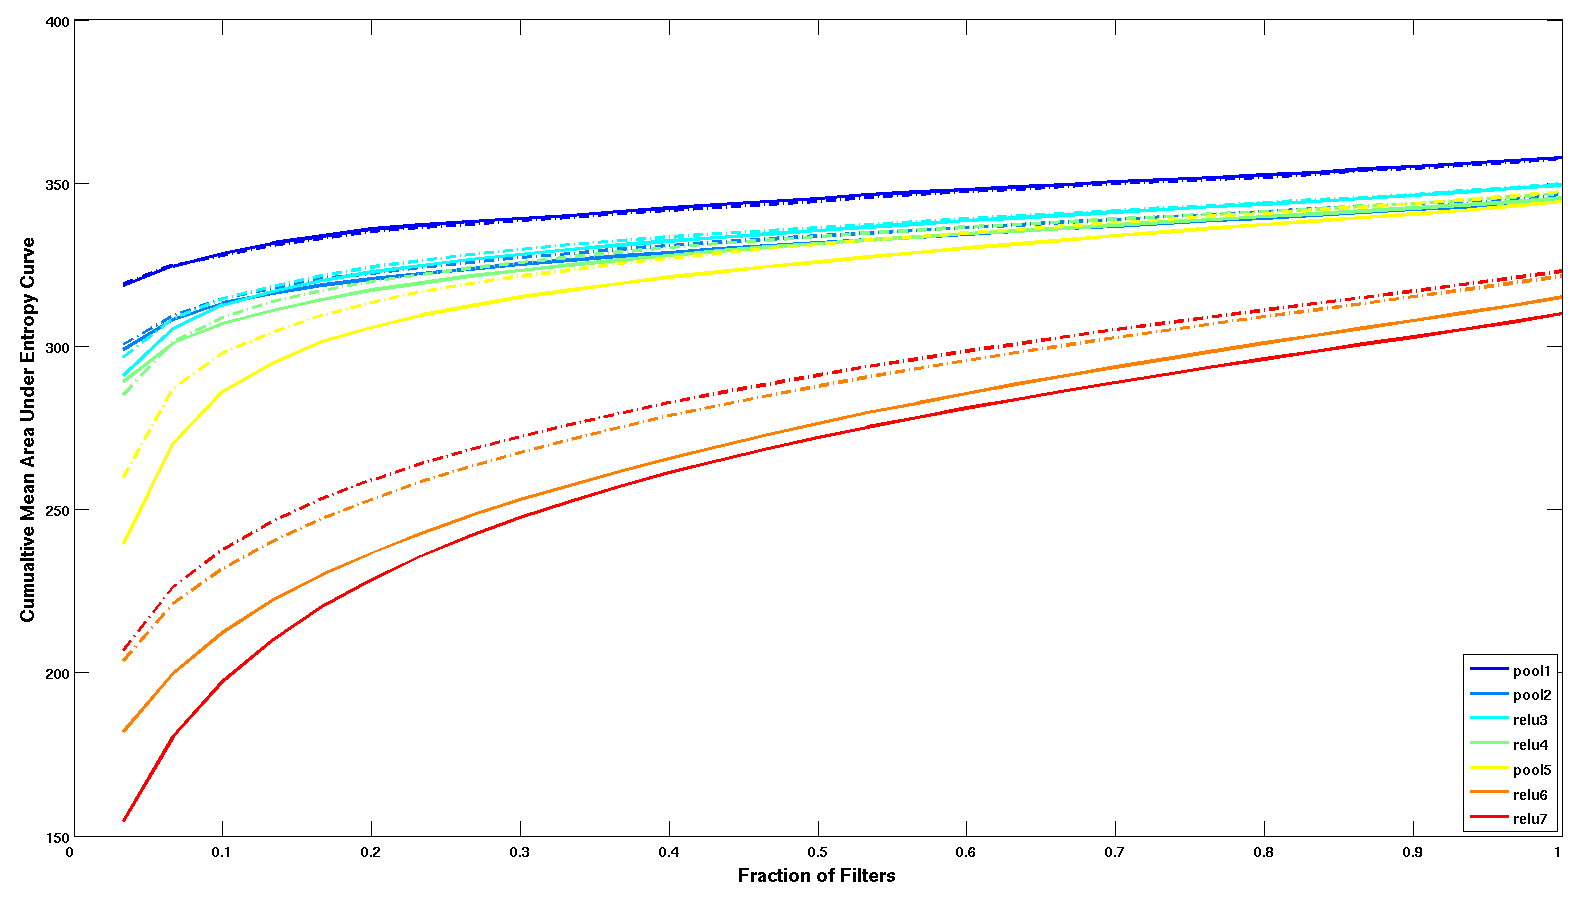
\includegraphics[scale=0.15]{images/weighted_layer_entropy.png}} \\
\subfloat{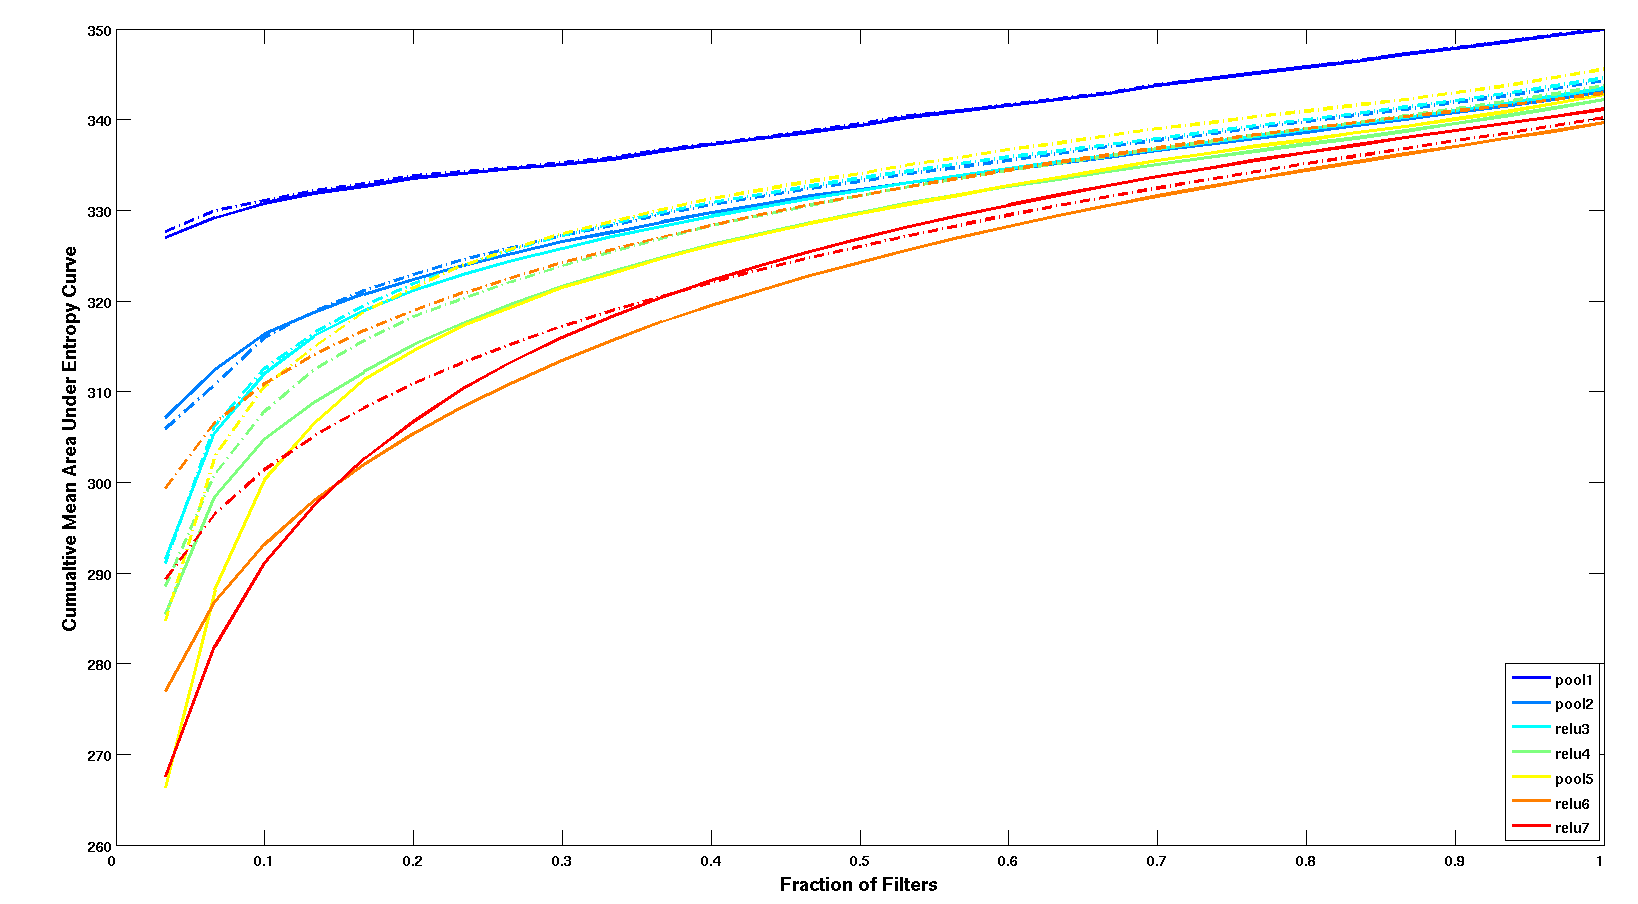
\includegraphics[scale=0.15]{images/spmax_layer_entropy.png}}
\caption{Mean Cumulative AuE plotted as fraction of filters for all layers of the Conv-Net. Dash-Dot Line: Alex-Net, Solid Line: Fine-Tuned Network. The top plot shows entropy calculated using Weighted Label-Entropy Method, whereas the bottom plot entropy calculated using spMax Label-Entropy Method.}
\label{fig:fine-entropy}
\end{figure}


\section{On Grand-Mother Cells}

\section{More Details on Training Setup} 



\bibliographystyle{splncs}
\bibliography{egbib}
\end{document}
